% Options for packages loaded elsewhere
\PassOptionsToPackage{unicode}{hyperref}
\PassOptionsToPackage{hyphens}{url}
\PassOptionsToPackage{dvipsnames,svgnames,x11names}{xcolor}
%
\documentclass[
  10pt,
  letterpaper,
  DIV=11,
  numbers=noendperiod]{scrartcl}

\usepackage{amsmath,amssymb}
\usepackage{lmodern}
\usepackage{iftex}
\ifPDFTeX
  \usepackage[T1]{fontenc}
  \usepackage[utf8]{inputenc}
  \usepackage{textcomp} % provide euro and other symbols
\else % if luatex or xetex
  \usepackage{unicode-math}
  \defaultfontfeatures{Scale=MatchLowercase}
  \defaultfontfeatures[\rmfamily]{Ligatures=TeX,Scale=1}
\fi
% Use upquote if available, for straight quotes in verbatim environments
\IfFileExists{upquote.sty}{\usepackage{upquote}}{}
\IfFileExists{microtype.sty}{% use microtype if available
  \usepackage[]{microtype}
  \UseMicrotypeSet[protrusion]{basicmath} % disable protrusion for tt fonts
}{}
\makeatletter
\@ifundefined{KOMAClassName}{% if non-KOMA class
  \IfFileExists{parskip.sty}{%
    \usepackage{parskip}
  }{% else
    \setlength{\parindent}{0pt}
    \setlength{\parskip}{6pt plus 2pt minus 1pt}}
}{% if KOMA class
  \KOMAoptions{parskip=half}}
\makeatother
\usepackage{xcolor}
\usepackage[top=10mm,left=15mm,left=15mm]{geometry}
\setlength{\emergencystretch}{3em} % prevent overfull lines
\setcounter{secnumdepth}{-\maxdimen} % remove section numbering
% Make \paragraph and \subparagraph free-standing
\ifx\paragraph\undefined\else
  \let\oldparagraph\paragraph
  \renewcommand{\paragraph}[1]{\oldparagraph{#1}\mbox{}}
\fi
\ifx\subparagraph\undefined\else
  \let\oldsubparagraph\subparagraph
  \renewcommand{\subparagraph}[1]{\oldsubparagraph{#1}\mbox{}}
\fi


\providecommand{\tightlist}{%
  \setlength{\itemsep}{0pt}\setlength{\parskip}{0pt}}\usepackage{longtable,booktabs,array}
\usepackage{calc} % for calculating minipage widths
% Correct order of tables after \paragraph or \subparagraph
\usepackage{etoolbox}
\makeatletter
\patchcmd\longtable{\par}{\if@noskipsec\mbox{}\fi\par}{}{}
\makeatother
% Allow footnotes in longtable head/foot
\IfFileExists{footnotehyper.sty}{\usepackage{footnotehyper}}{\usepackage{footnote}}
\makesavenoteenv{longtable}
\usepackage{graphicx}
\makeatletter
\def\maxwidth{\ifdim\Gin@nat@width>\linewidth\linewidth\else\Gin@nat@width\fi}
\def\maxheight{\ifdim\Gin@nat@height>\textheight\textheight\else\Gin@nat@height\fi}
\makeatother
% Scale images if necessary, so that they will not overflow the page
% margins by default, and it is still possible to overwrite the defaults
% using explicit options in \includegraphics[width, height, ...]{}
\setkeys{Gin}{width=\maxwidth,height=\maxheight,keepaspectratio}
% Set default figure placement to htbp
\makeatletter
\def\fps@figure{htbp}
\makeatother

\KOMAoption{captions}{tableheading}
\makeatletter
\makeatother
\makeatletter
\makeatother
\makeatletter
\@ifpackageloaded{caption}{}{\usepackage{caption}}
\AtBeginDocument{%
\ifdefined\contentsname
  \renewcommand*\contentsname{Table of contents}
\else
  \newcommand\contentsname{Table of contents}
\fi
\ifdefined\listfigurename
  \renewcommand*\listfigurename{List of Figures}
\else
  \newcommand\listfigurename{List of Figures}
\fi
\ifdefined\listtablename
  \renewcommand*\listtablename{List of Tables}
\else
  \newcommand\listtablename{List of Tables}
\fi
\ifdefined\figurename
  \renewcommand*\figurename{Figure}
\else
  \newcommand\figurename{Figure}
\fi
\ifdefined\tablename
  \renewcommand*\tablename{Table}
\else
  \newcommand\tablename{Table}
\fi
}
\@ifpackageloaded{float}{}{\usepackage{float}}
\floatstyle{ruled}
\@ifundefined{c@chapter}{\newfloat{codelisting}{h}{lop}}{\newfloat{codelisting}{h}{lop}[chapter]}
\floatname{codelisting}{Listing}
\newcommand*\listoflistings{\listof{codelisting}{List of Listings}}
\makeatother
\makeatletter
\@ifpackageloaded{caption}{}{\usepackage{caption}}
\@ifpackageloaded{subcaption}{}{\usepackage{subcaption}}
\makeatother
\makeatletter
\@ifpackageloaded{tcolorbox}{}{\usepackage[many]{tcolorbox}}
\makeatother
\makeatletter
\@ifundefined{shadecolor}{\definecolor{shadecolor}{rgb}{.97, .97, .97}}
\makeatother
\makeatletter
\makeatother
\ifLuaTeX
  \usepackage{selnolig}  % disable illegal ligatures
\fi
\IfFileExists{bookmark.sty}{\usepackage{bookmark}}{\usepackage{hyperref}}
\IfFileExists{xurl.sty}{\usepackage{xurl}}{} % add URL line breaks if available
\urlstyle{same} % disable monospaced font for URLs
\hypersetup{
  colorlinks=true,
  linkcolor={EF58A0},
  filecolor={Maroon},
  citecolor={Blue},
  urlcolor={Blue},
  pdfcreator={LaTeX via pandoc}}

\author{}
\date{}

\begin{document}
\ifdefined\Shaded\renewenvironment{Shaded}{\begin{tcolorbox}[breakable, boxrule=0pt, frame hidden, borderline west={3pt}{0pt}{shadecolor}, enhanced, interior hidden, sharp corners]}{\end{tcolorbox}}\fi

Luis \textbf{Sarmiento} \vspace{-0.15cm}

Environmental Economist

\vspace{-0.25cm}

\noindent 

\rule{5cm}{1pt}
\vspace{0.25cm}


\includegraphics[width=1em,height=1em]{cv_pdf_files/figure-pdf/fa-icon-f25e429b6e525c94655c4c1ea9a89fbd.pdf}
luissarmiento.com \vspace{-0.15cm}


\includegraphics[width=1em,height=1em]{cv_pdf_files/figure-pdf/fa-icon-0472185263d085cbc13489893c2b12dc.pdf}
gsaabogado@gmail.com \vspace{-0.15cm}


\includegraphics[width=0.88em,height=1em]{cv_pdf_files/figure-pdf/fa-icon-65ad8d20d25bdcf13492029ffb936540.pdf}
\href{https://www.linkedin.com/in/luis-sarmiento-eco}{luis-sarmiento-eco}
\vspace{-0.15cm}


\includegraphics[width=0.75em,height=1em]{cv_pdf_files/figure-pdf/fa-icon-007427b345eb0c895578b1173ef82880.pdf}
+39 030 897890 \vspace{-0.15cm}


\includegraphics[width=0.75em,height=1em]{cv_pdf_files/figure-pdf/fa-icon-73878e667d08a27804bf0774c72de1fb.pdf}
Via Bergognone, 34, 20144 Milan MI, Italy \vspace{-0.15cm}

\vspace{0.5 cm}

Applied economist focusing on \textbf{causal inference} and
\textbf{energy modelling}.

\hypertarget{work-experience}{%
\subsection[ Work Experience
\vspace{-0.5cm}]{\texorpdfstring{\protect
\includegraphics[width=1em,height=1em]{cv_pdf_files/figure-pdf/fa-icon-65a83bdea6161284dcc1b960352dd7dd.pdf}
Work Experience
\vspace{-0.5cm}}{ Work Experience }}\label{work-experience}}

\hrulefill

\vspace{-0.15cm}

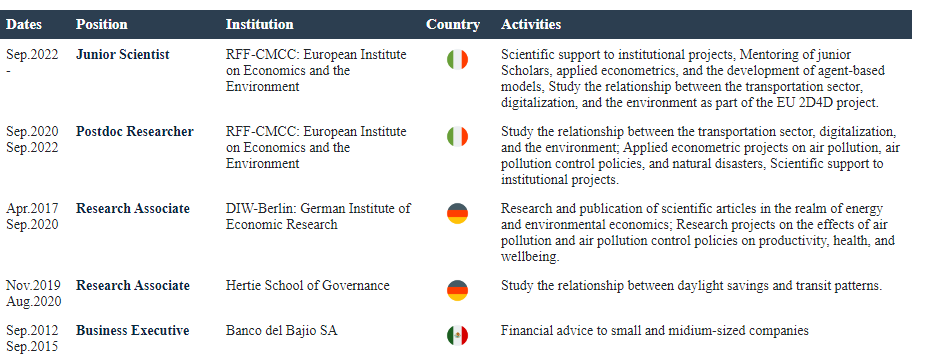
\includegraphics{cv_pdf_files/figure-pdf/unnamed-chunk-1-1.png}

\hypertarget{education}{%
\subsection[ Education
\vspace{-0.5cm}]{\texorpdfstring{\protect
\includegraphics[width=1em,height=1em]{cv_pdf_files/figure-pdf/fa-icon-2d63498385de2eb86c2b263aaf24cf57.pdf}
Education \vspace{-0.5cm}}{ Education }}\label{education}}

\hrulefill

\vspace{-0.15cm}

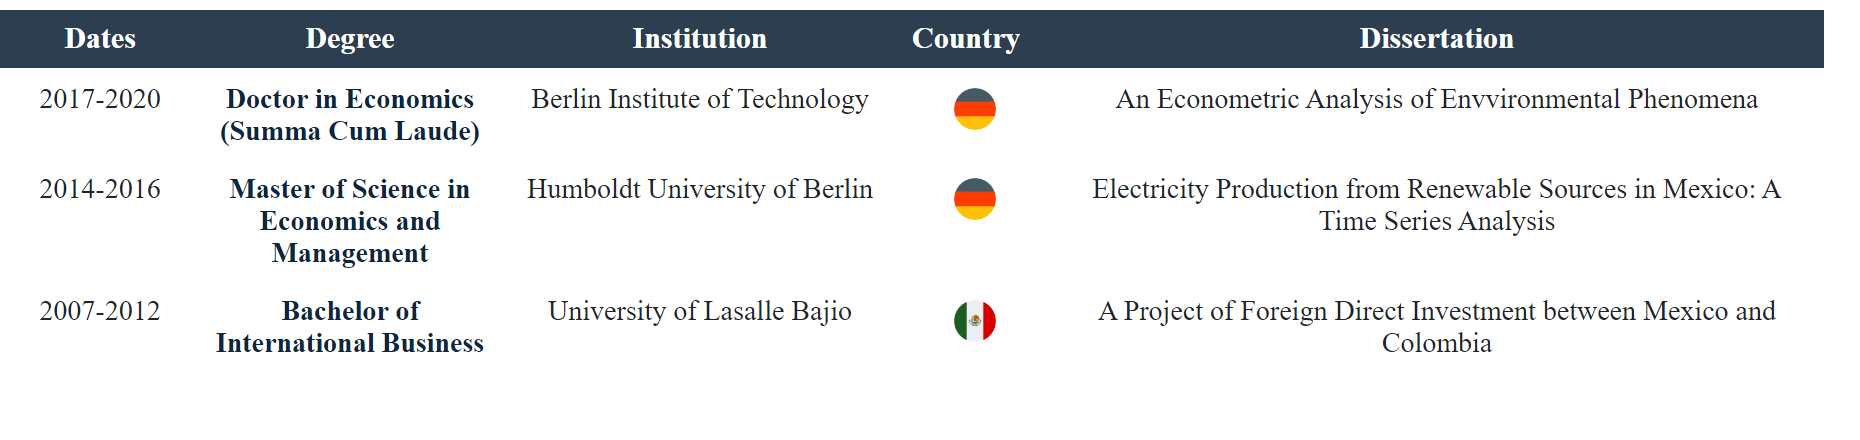
\includegraphics{cv_pdf_files/figure-pdf/unnamed-chunk-2-1.png}

\hypertarget{research-interests}{%
\subsubsection[ Research
Interests]{\texorpdfstring{\protect
\includegraphics[width=1.12em,height=1em]{cv_pdf_files/figure-pdf/fa-icon-36bc015840b9f29e0796dd871d58fbdb.pdf}
Research Interests}{ Research Interests}}\label{research-interests}}

\begin{table}[H]
\centering\begingroup\fontsize{10.5}{12.5}\selectfont

\resizebox{\linewidth}{!}{
\begin{tabular}{>{\raggedleft\arraybackslash}p{12em}>{\raggedright\arraybackslash}p{52.5em}}
\toprule
\cellcolor{gray!6}{\textbf{Applied Econometrics}} & \cellcolor{gray!6}{Use of econometric methods for causal inference}\\
\textbf{Digitalization and the Environment} & Analysis of the inter-dependenencies between the transportation sector, digitalization, and the environment\\
\cellcolor{gray!6}{\textbf{Energy Modeling}} & \cellcolor{gray!6}{Design and Implementation of optimization models to assess public policies for the decabornization of energy systems}\\
\textbf{Agent Based Models} & Design and implementation of agent-based models to understand households' adoption of green technologies\\
\bottomrule
\end{tabular}}
\endgroup{}
\end{table}

\hypertarget{softwares-and-lenguages}{%
\subsection[ Softwares and
Lenguages]{\texorpdfstring{\protect
\includegraphics[width=1.25em,height=1em]{cv_pdf_files/figure-pdf/fa-icon-22b8f3417d46c1380415023f37fb9d64.pdf}
Softwares and
Lenguages}{ Softwares and Lenguages}}\label{softwares-and-lenguages}}

\begin{figure}

\begin{minipage}[t]{0.50\linewidth}

{\centering 

\raisebox{-\height}{

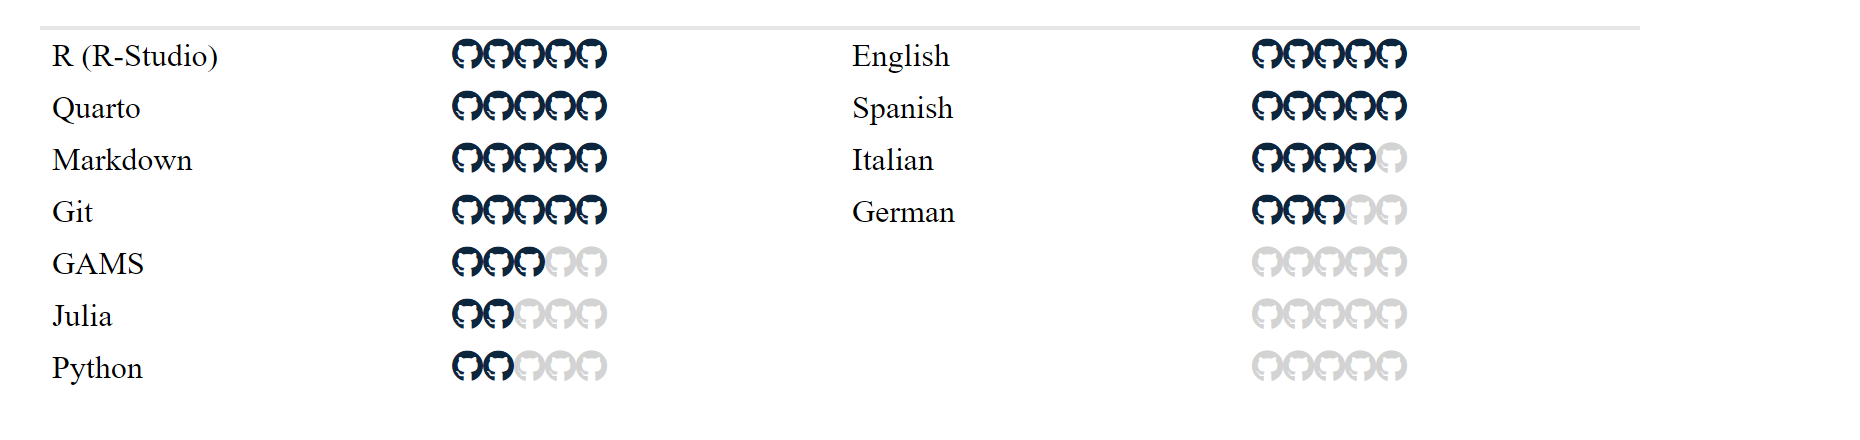
\includegraphics{cv_pdf_files/figure-pdf/unnamed-chunk-4-1.png}

}

}

\end{minipage}%

\end{figure}



\end{document}
